\documentclass[professionalfont]{beamer}

\usepackage{graphicx}
\usepackage{newtxtext,newtxmath}
\usepackage[backend=bibtex]{biblatex} 
\addbibresource{ref.bib}
\renewcommand*{\bibfont}{\scriptsize}

\usetheme{default}
\usecolortheme{seagull}

\setbeamertemplate{navigation symbols}{}
\setbeamertemplate{itemize item}{\textbullet} 
\setbeamertemplate{bibliography item}[text]
\setbeamertemplate{title page}{
    \begin{center}
        {\textcolor{blue}{\textbf{\fontsize{13}{14}\selectfont
        Attention Is All You Need}}} \\[1.5cm]
        
        {\fontsize{9}{14}\selectfont Ashish Vaswani, et al \\[0.3cm]
        Google \\[0.3cm]
        NeurIPS 2017}
    \end{center}
}
% ------------------ Title ------------------

\begin{document}
\frame{\titlepage}

% ------------------ Slide 1 ------------------

\begin{frame}
\begin{center}
    { \textbf{\textcolor{blue}{ {\fontsize{12}{14}\selectfont Abstract} }} }
\end{center}
\\[0.3cm]

{\fontsize{10}{14}\selectfont 
\begin{itemize}
    \item Prior works for sequence transduction
    
    - RNN: hard to parallelize due to sequential dependencies

    - CNN: lack of long-range dependencies due to fixed window

    \\[0.5cm]

    \item Transformer: New simple architecture

    - It is purely based on attention

    - It can process sequences in parallel
    
    - It has global context understanding

    \\[0.5cm]

    \item Performance

    - SOTA on English to German, French tasks

    - It is faster to train, not only better performance

    - It generalizes well to other tasks
\end{itemize}
}

\end{frame}

% ------------------ Slide 2 ------------------

\begin{frame}

\begin{center}
    { \textbf{\textcolor{blue}{ {\fontsize{12}{14}\selectfont Framework} }} }
\end{center}
\\[0.2cm]

\begin{columns}
\column{0.5\textwidth}
    {\fontsize{10}{14}\selectfont
        \begin{itemize}
            \item Encoder stack
    
            - Input \( \textbf{x} \) to representation \( \textbf{z} \)

            - Multihead attention

            \\[0.3cm]
            
            \item Decoder stack
    
            - Given \( \textbf{z} \), output \( \textbf{y} \)

            - Masked attention

            - Encoder-Decoder attention

            \\[0.3cm]

            \item Common component

            - Stack of \( N=6 \) identical layers

            - Dimension is \( d_{model} = 512 \)

            - LayerNorm \& Residual

            - Fully connected FFN
\end{itemize}
}
\column{0.5\textwidth}
    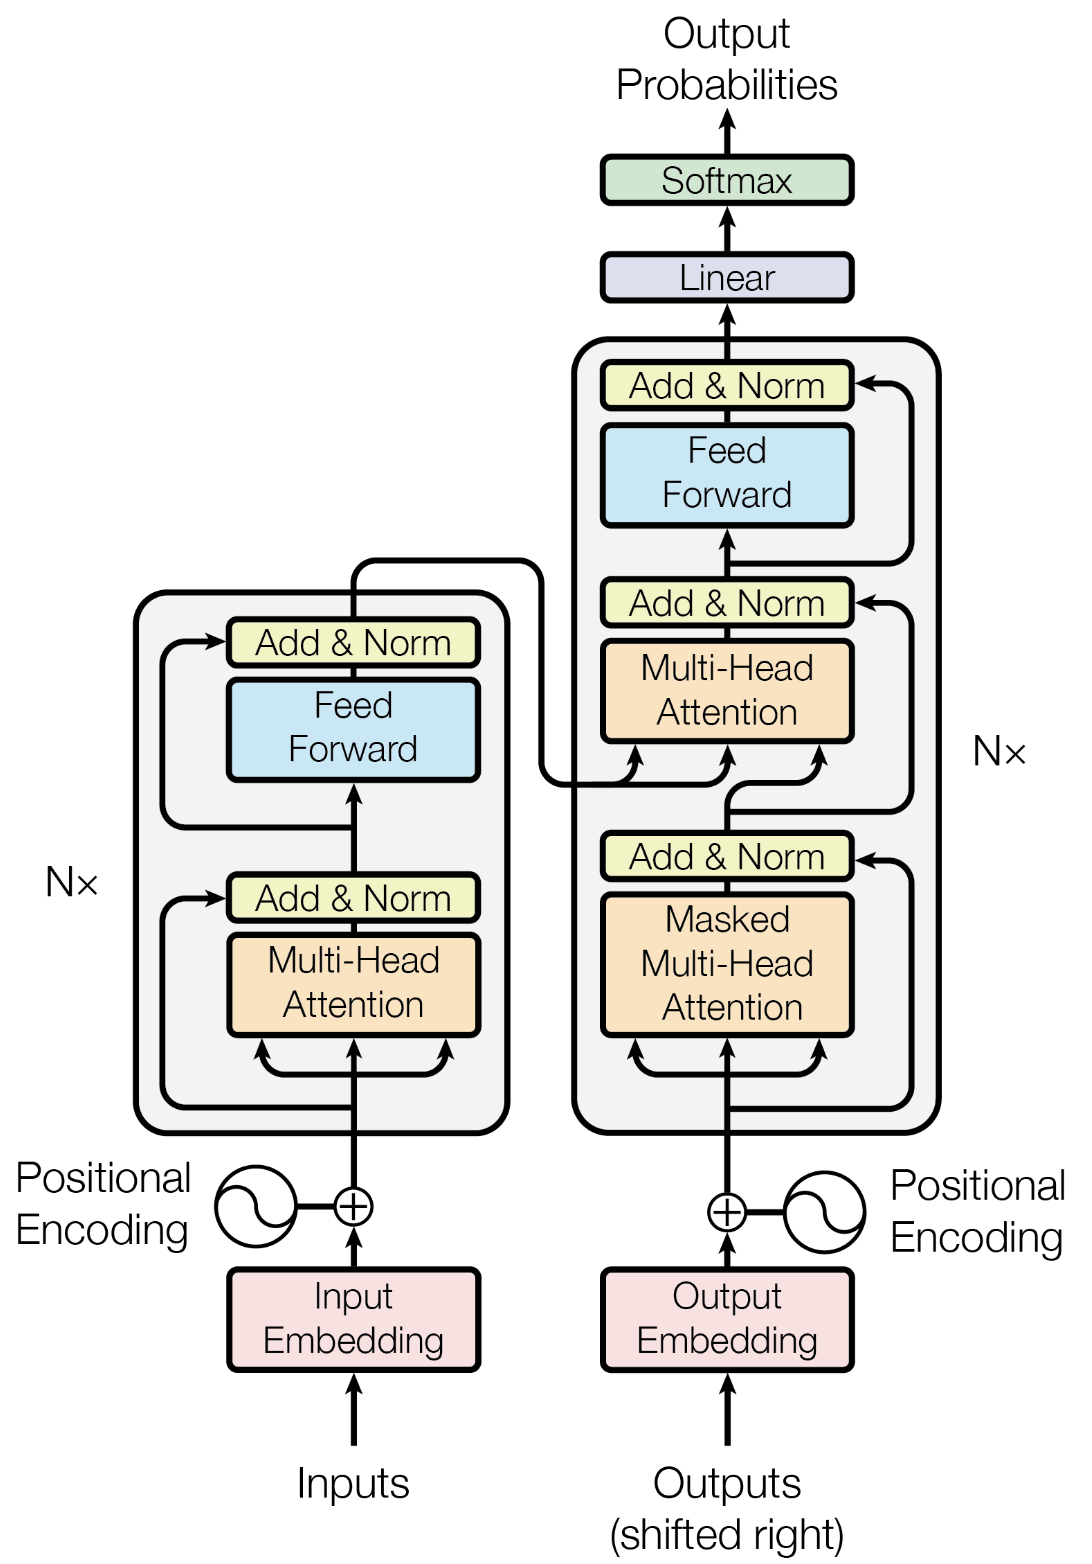
\includegraphics[width=1.0\linewidth]{figure/1.png}
\end{columns}

\end{frame}
% ------------------ Slide 3 ------------------

\begin{frame}

\begin{center}
    { \textbf{\textcolor{blue}{ {\fontsize{12}{14}\selectfont Framework} }} }
\end{center}
\\[0.2cm]

\begin{center}
    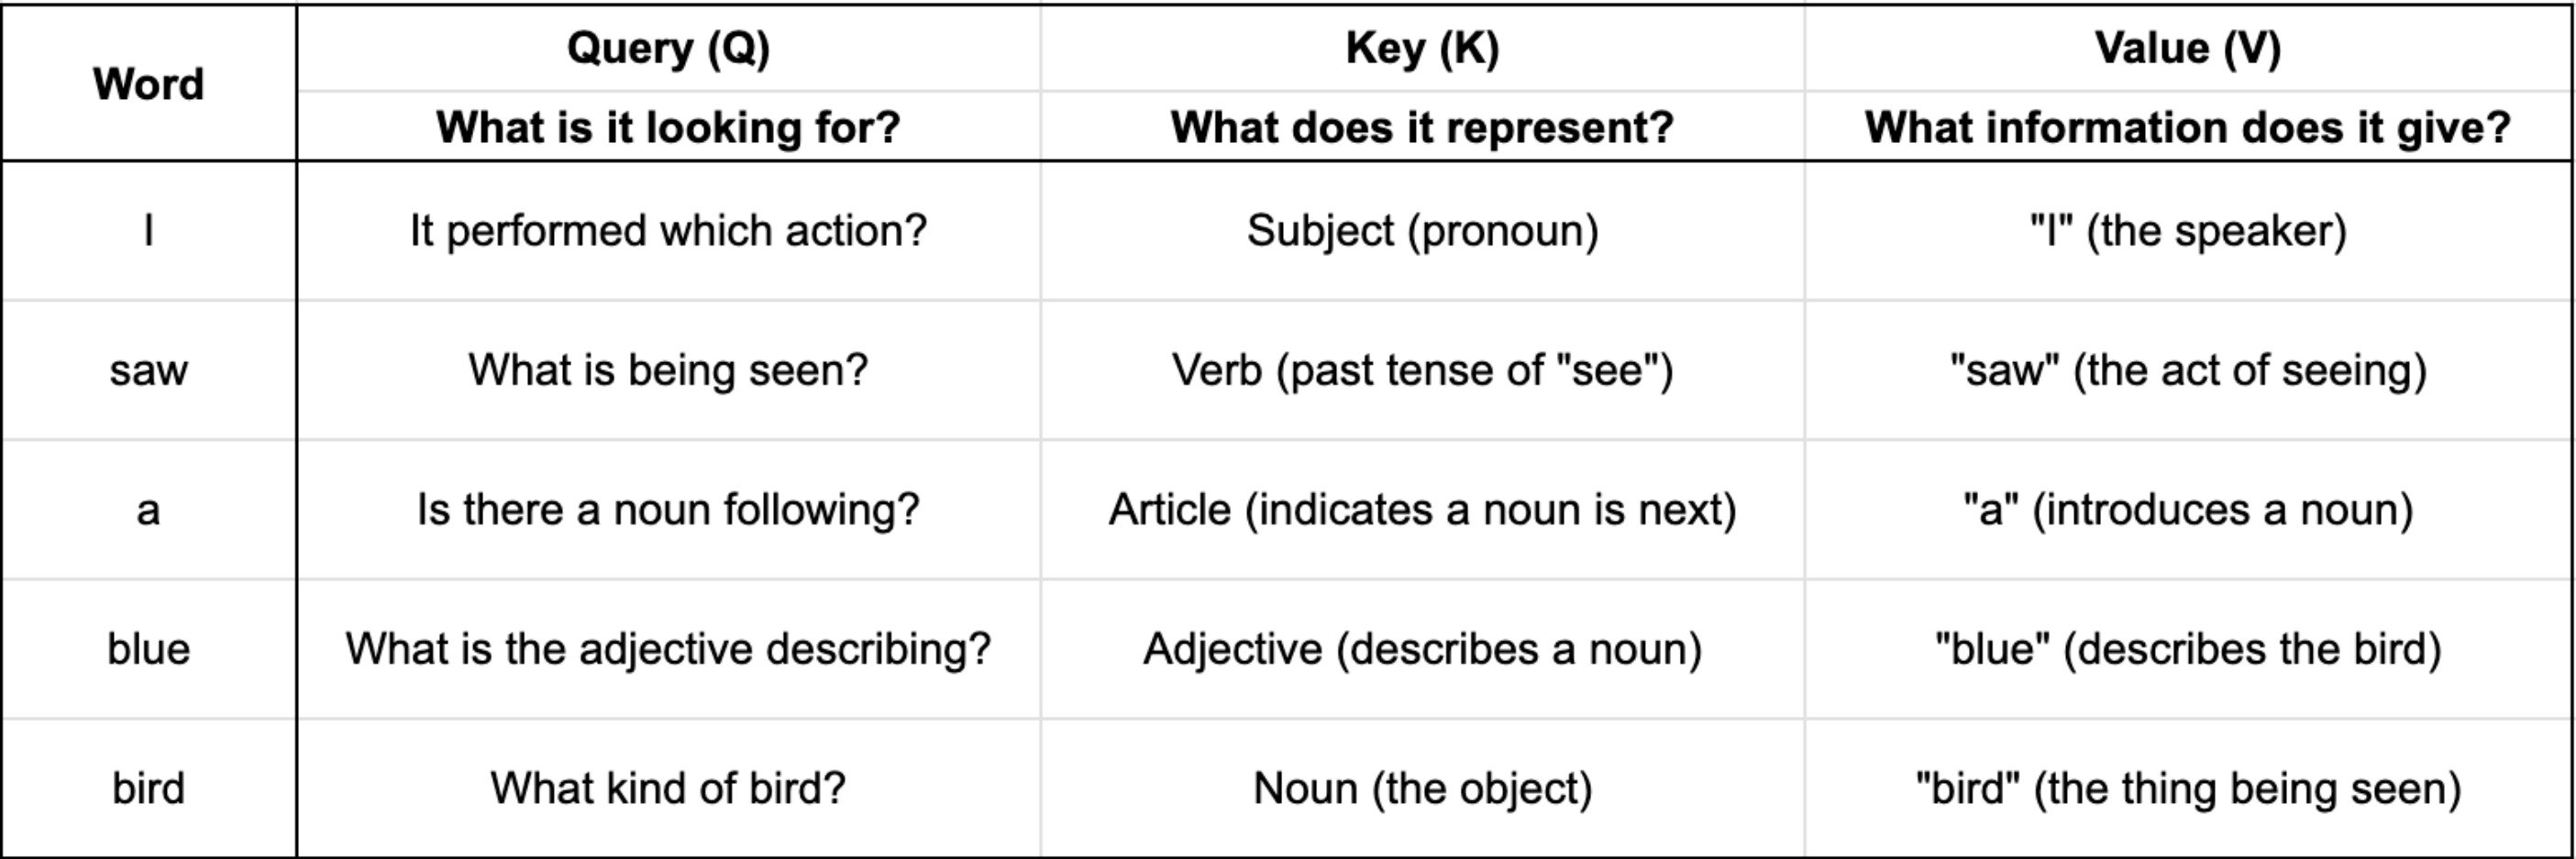
\includegraphics[width=1.0\textwidth]{custom/1.png}
\end{center}

\begin{itemize}
    \item Scaled Dot-Product Attention

    - Query \(Q\), Key \(K\), Value \(V\)

    - Attention\( (Q, K, V) = \) softmax\( (\frac{QK^T}{\sqrt{d_k}})V \)

    - Large \( d_k \) causes extreme softmax outputs

    - Scaling to prevent vanishing gradient
\end{itemize}

\end{frame}
% ------------------ Slide 4 ------------------

\begin{frame}

\begin{center}
    { \textbf{\textcolor{blue}{ {\fontsize{12}{14}\selectfont Framework} }} }
\end{center}
\\[0.2cm]

\begin{center}
    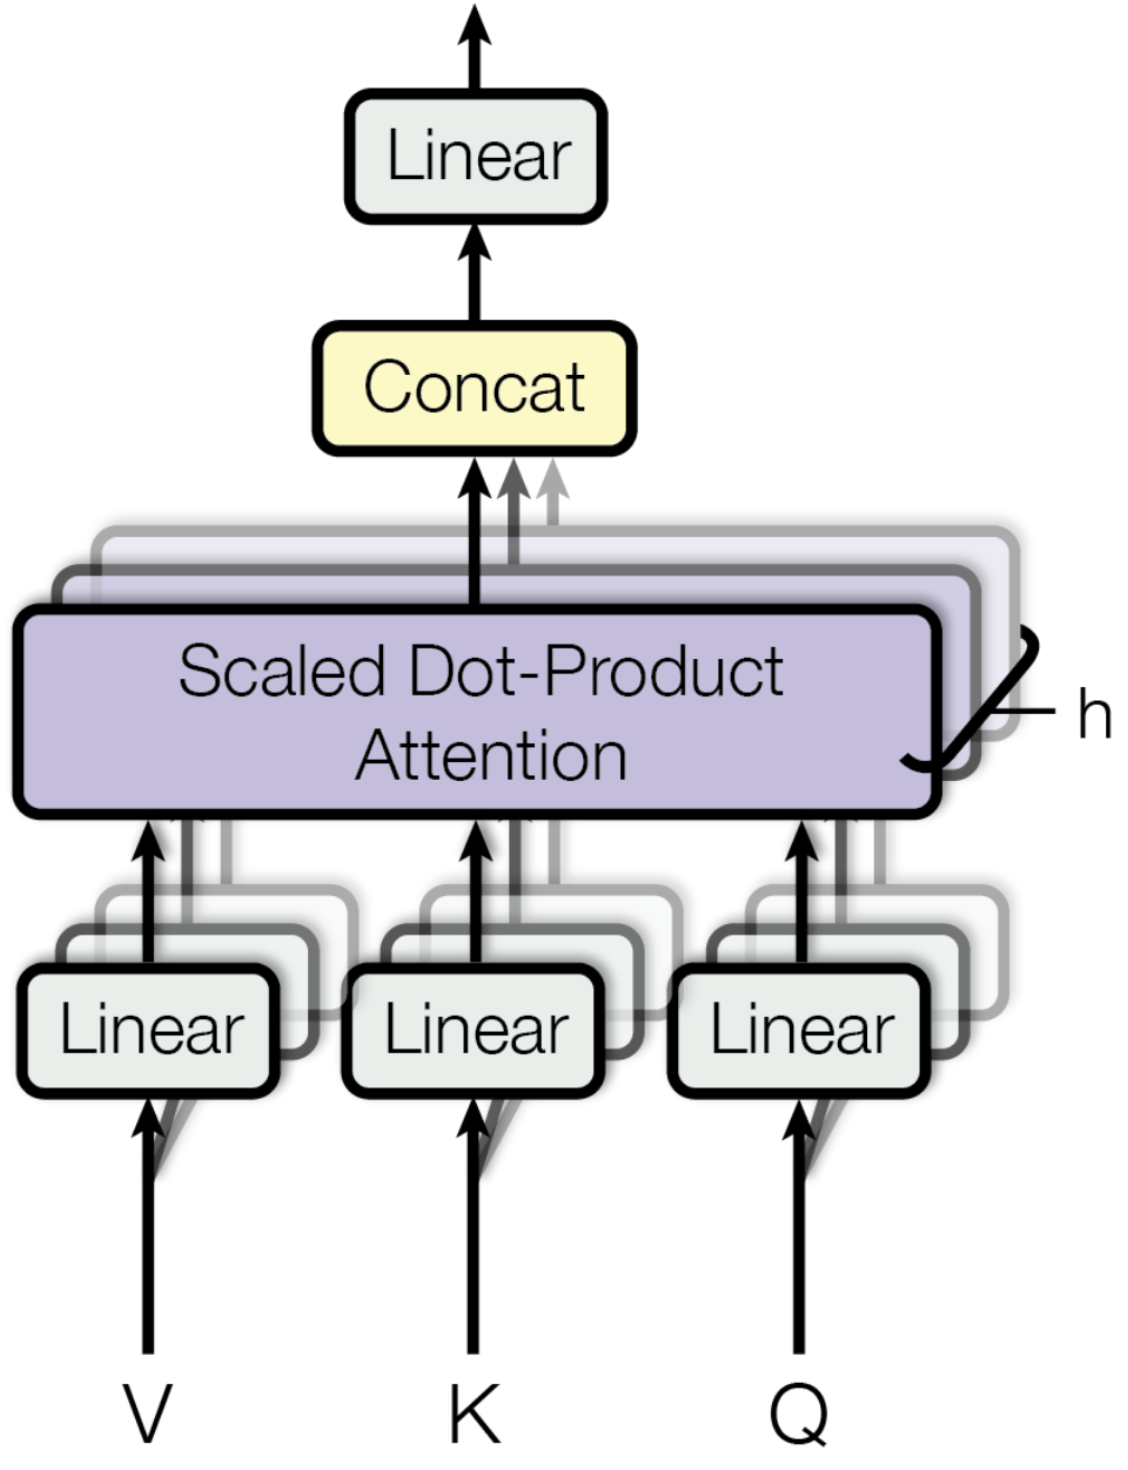
\includegraphics[width=0.3\textwidth]{figure/2.png}
\end{center}

\begin{itemize}
    \item Multi-Head Attention \( (h=8) \)

    - MultiHead\( (Q,K,V) = \) Concat\( (head_1, \cdots , head_h)W^O \)

    - \( head_i = \) Attention\( (QW_i^Q, KW_i^K, VW_i^V) \)

    - Each head focuses on different aspects of relationships
\end{itemize}

\end{frame}
% ------------------ Slide 5 ------------------

\begin{frame}

\begin{center}
    { \textbf{\textcolor{blue}{ {\fontsize{12}{14}\selectfont Framework} }} }
\end{center}
\\[0.2cm]

\begin{itemize}
    \item Self Attention

    - Helps each word attend to all other words

    - Long-range dependency \& Parallelizable

    \\[0.4cm]

    \item Masked Self Attention

    - During training, also parallelizable

    - Decoder must only attends to previous tokens

    - Future token attention scores are \( -\infty \)

    \\[0.4cm]

    \item Encoder-Decoder Attention

    - Decoder focus on relevant parts of the input context

    - It acts as a bridge between the encoder and decoder
\end{itemize}

\end{frame}
% ------------------ Slide 6 ------------------


\begin{frame}

\begin{center}
    { \textbf{\textcolor{blue}{ {\fontsize{12}{14}\selectfont Framework} }} }
\end{center}
\\[0.5cm]

\begin{itemize}
    \item Position-wise Feed-Forward Networks

    - \( FFN(x) = ReLU(xW_1+b_1)W_2 + b_2 \)

    - Input, Output dimension is 512

    - Inner-layer's dimension is 2048

    \\[0.5cm]

    \item Positional Encoding

    - \( PE_{(pos,2i)} = sin(pos/10000^{2i/d_{model}}) \)

    - \( PE_{(pos,2i+1)} = cos(pos/10000^{2i/d_{model}}) \)

    - Transformer doesn't process tokens sequentially

    - It can't distinguish ``I go to school" and ``to I school go"

    - Learned encoding is slightly better but costly
\end{itemize}

\end{frame}
% ------------------ Slide 7 ------------------

\begin{frame}
\begin{center}
    { \textbf{\textcolor{blue}{ {\fontsize{12}{14}\selectfont Why Self-Attention} }} }
\end{center}
\\[0.3cm]

\hrule

\begin{table}[]
\begin{tabular}{ccc}
\textbf{Type} & \textbf{Computational Complexity} & \textbf{Path Length} \\
RNN & O(n) & O(n) \\
CNN & O(kn) & O(log n) \\
Transformer & O(n^2) & O(1)
\end{tabular}
\end{table}

\hrule
\vspace{0.3cm}

{\fontsize{10}{14}\selectfont 
\begin{itemize}
    \item Computational Complexity

    - Transformer's matrix multiplications are expensive

    - However, it is parallelizable, making it faster than others

    - When \( n \) is very large, restricted window may be used

    \\[0.2cm]

    \item Path Length for Long-Range Dependencies

    - Each word attends to every other word directly

    \\[0.2cm]

    \item Interpretability

    - Some heads focus on syntax, others focus on semantics
\end{itemize}
}

\end{frame}
% ------------------ Slide 8 ------------------

\begin{frame}
\begin{center}
    { \textbf{\textcolor{blue}{ {\fontsize{12}{14}\selectfont Training} }} }
\end{center}
\\[0.3cm]

{\fontsize{10}{14}\selectfont 
\begin{itemize}
    \item Dataset

    - English to German translation

    - English to French translation

    \\[0.4cm]
    
    \item Hardware and schedule

    - 8 NVIDIA P100 GPUs (2017 top GPUs)

    - Base model: 100K steps (12 hours)

    - Big model: 300K steps (3.5 days)
\end{itemize}
}

\end{frame}
% ------------------ Slide 9 ------------------

\begin{frame}

\begin{center}
    { \textbf{\textcolor{blue}{ {\fontsize{12}{14}\selectfont Results} }} }
\end{center}
\\[0.3cm]

\begin{center}
    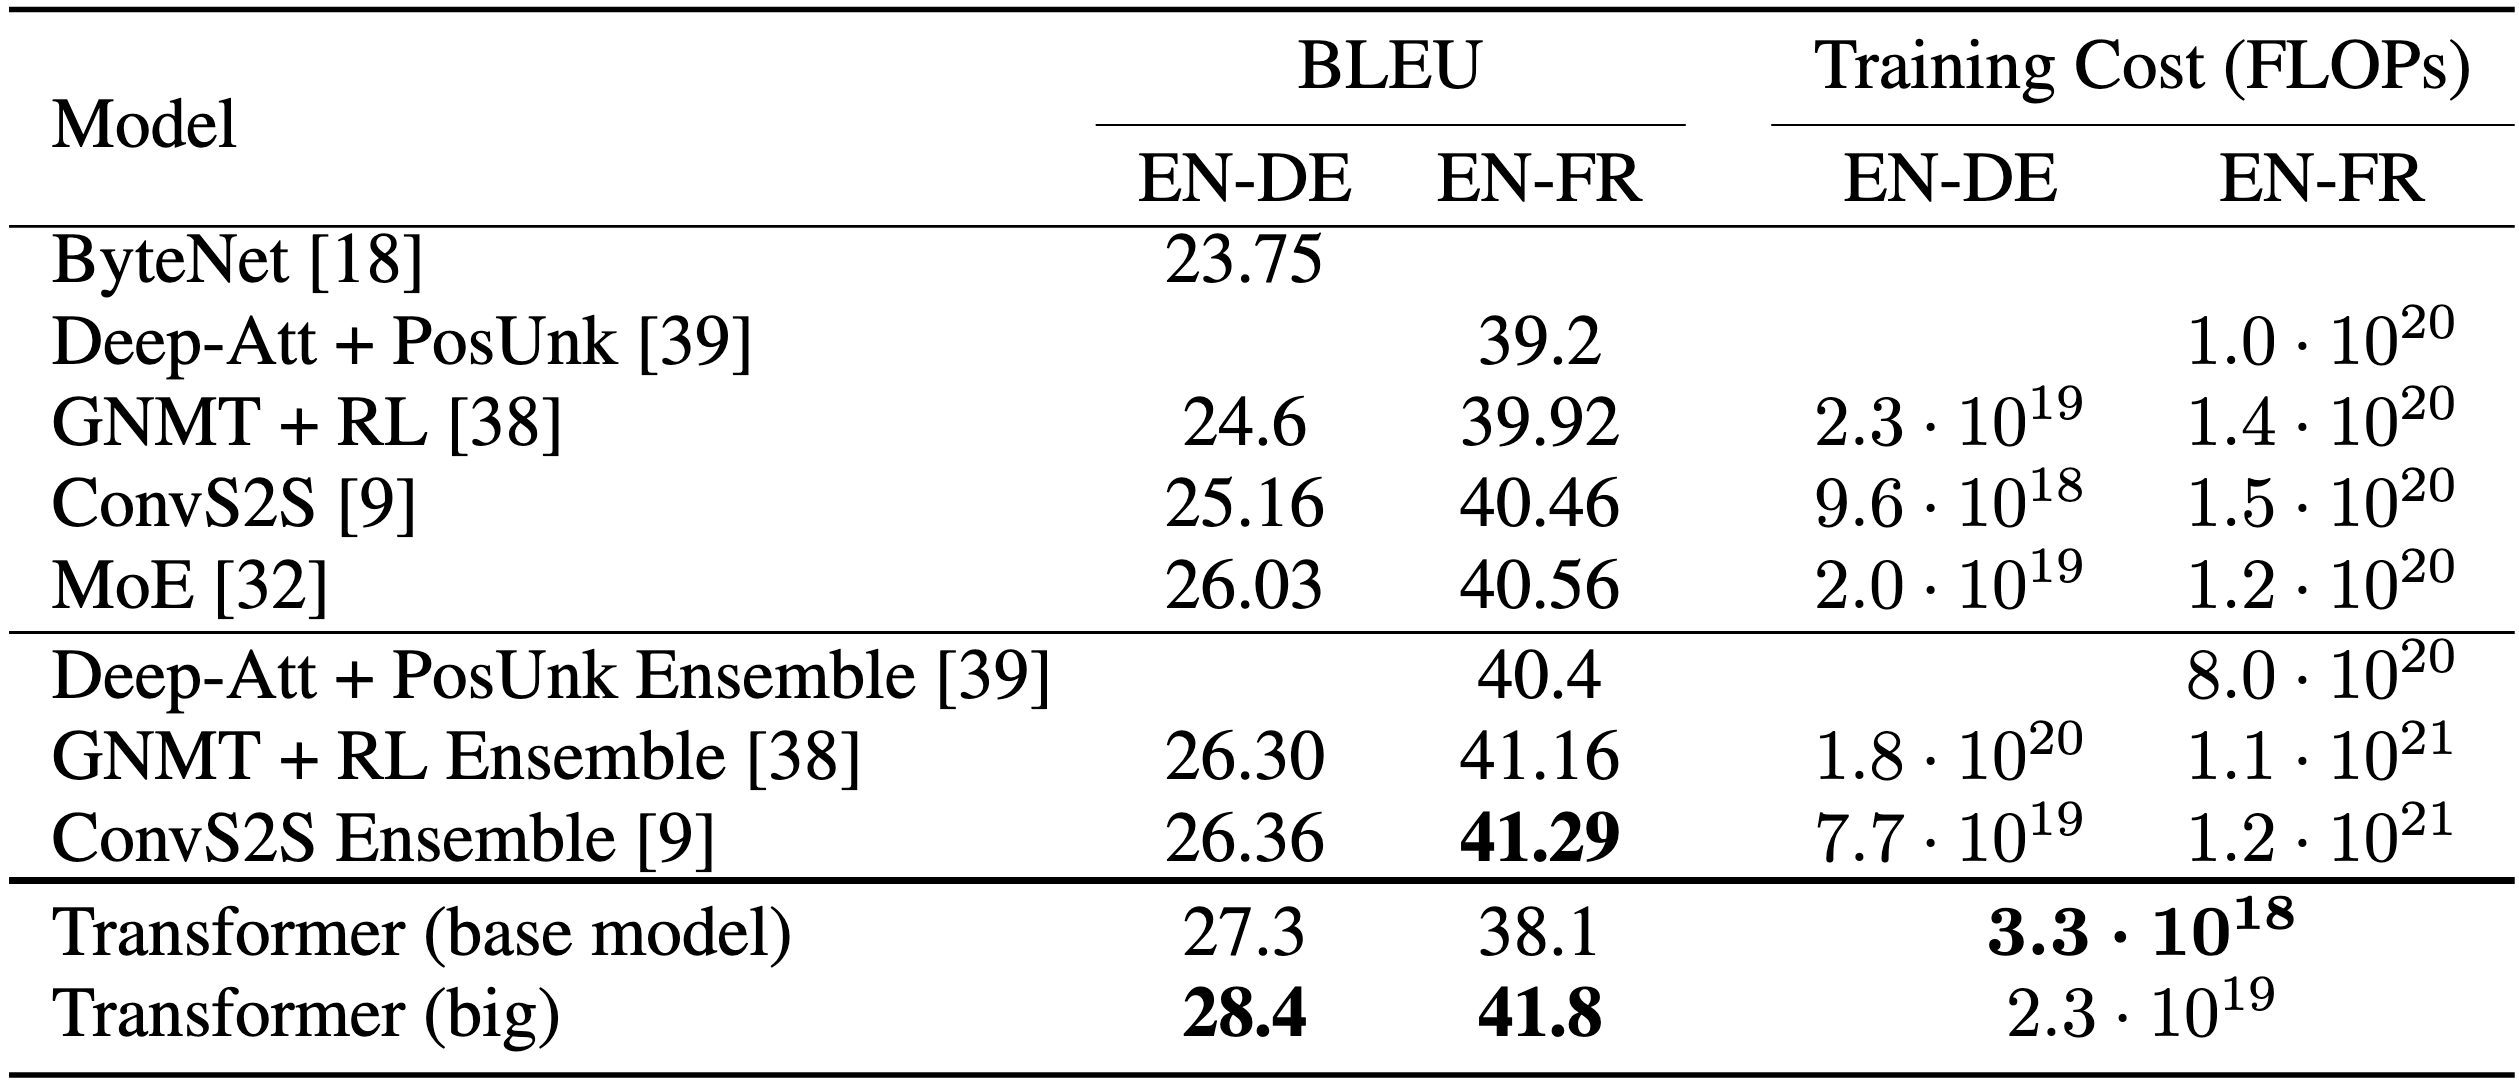
\includegraphics[width=1.0\textwidth]{table/2.png}
\end{center}

{\fontsize{10}{14}\selectfont 
\begin{itemize}
    \item Machine translation task

    - Transformer outperformed all previous models, even ensembles

    - Trains much faster than previous models (3.5 days vs. weeks)

\end{itemize}
}

\end{frame}
% ------------------ Slide 10 ------------------

\begin{frame}

\begin{center}
    { \textbf{\textcolor{blue}{ {\fontsize{12}{14}\selectfont Results} }} }
\end{center}

\begin{center}
    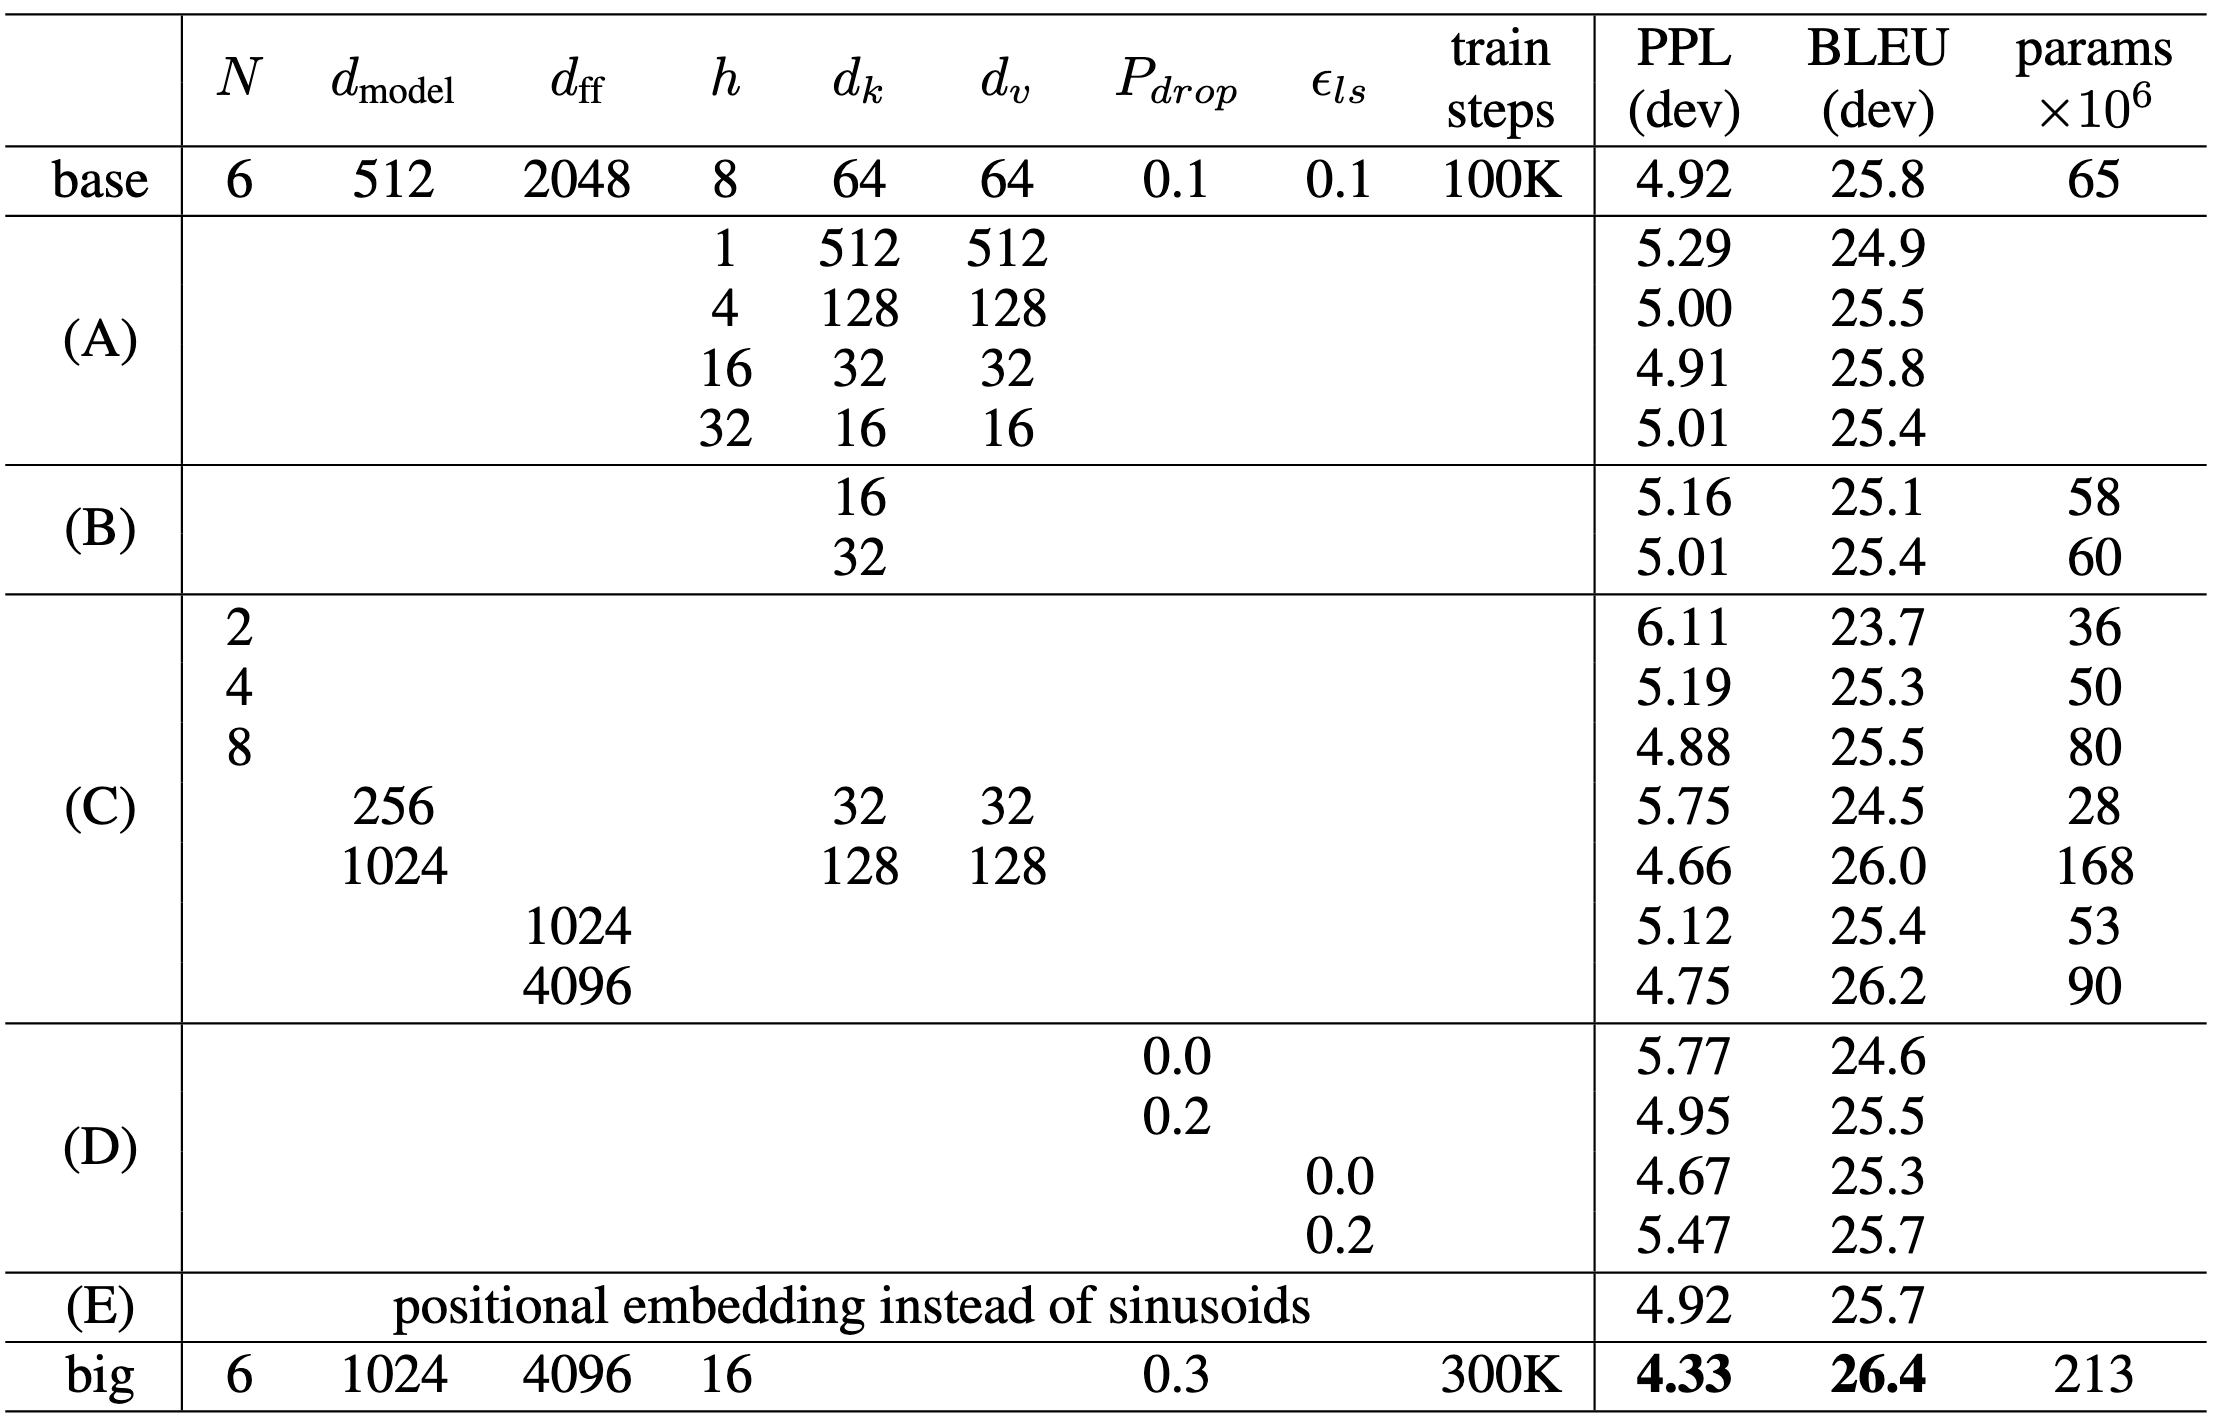
\includegraphics[width=0.7\textwidth]{table/3.png}
\end{center}

{\fontsize{10}{14}\selectfont 
\begin{itemize}
    \item Ablation

    - Optimal number of heads exists

    - Higher dimension, Larger model size is better

    - Dropout is effective, Learned PE is not effective

\end{itemize}
}

\end{frame}
% ------------------ Slide 11 ------------------

\begin{frame}
\begin{refsection}

\begin{center}
    { \textbf{\textcolor{blue}{ {\fontsize{12}{14}\selectfont Analysis} }} }
\end{center}
\\[0.2cm]

\begin{center}
    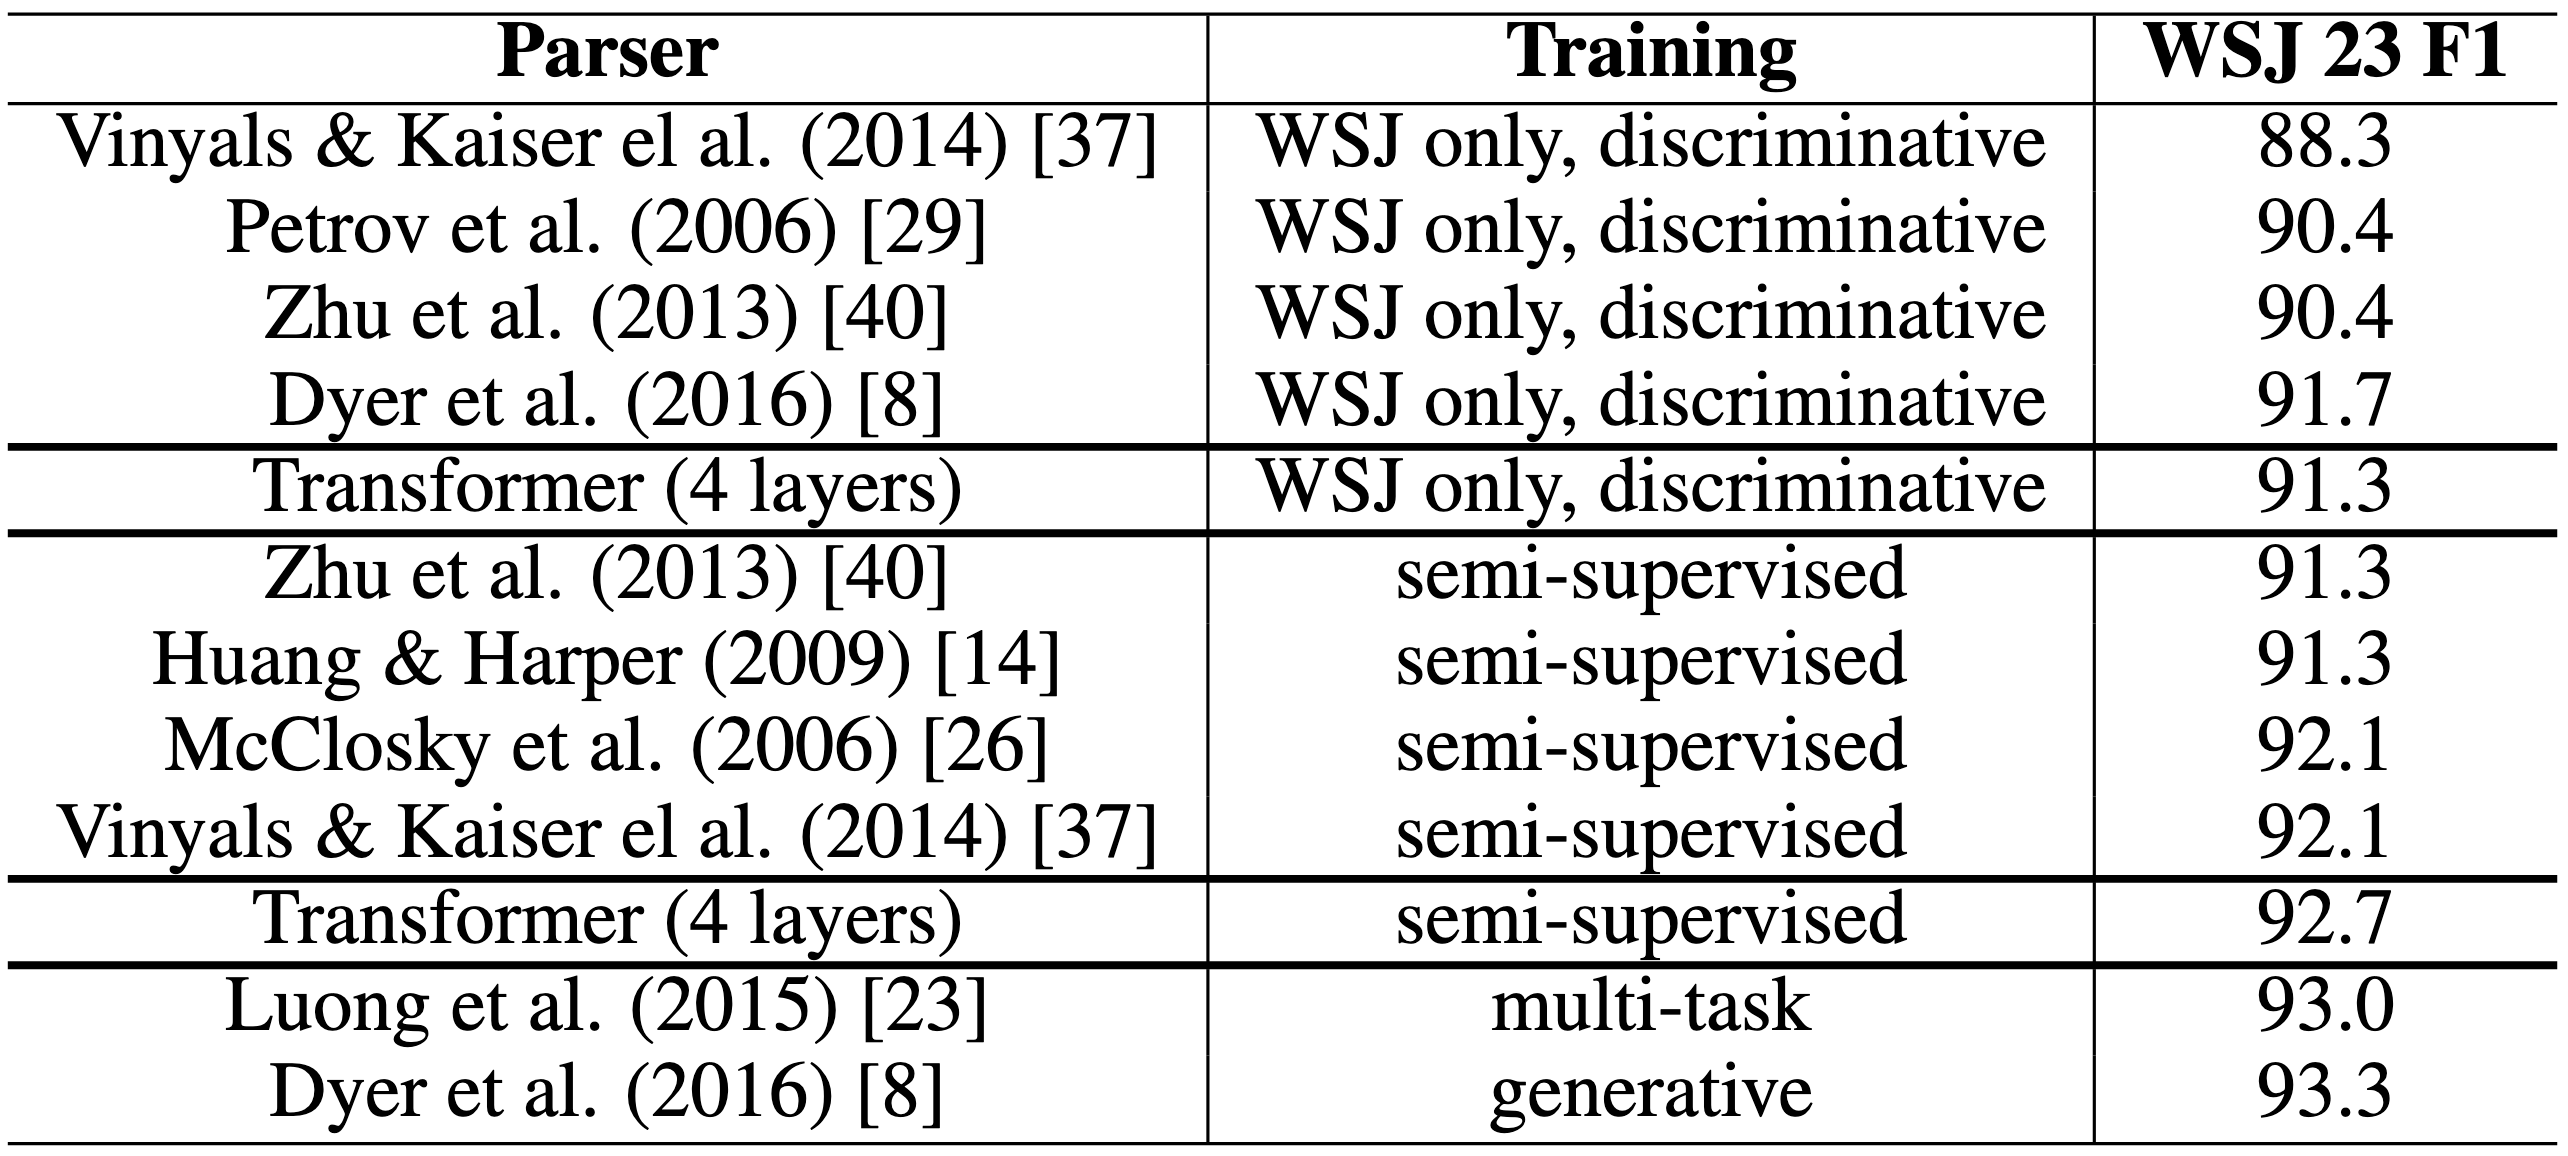
\includegraphics[width=0.8\textwidth]{table/4.png}
\end{center}

{\fontsize{10}{14}\selectfont 
\begin{itemize}
    \item English Constituency Parsing (Analyzing syntax)

    - Small dataset: Wall Street Journal (40K Sentences)

    - Large dataset: Semi-supervised setting (17M Sentences)

    - Close to RNNG, the SOTA \cite{RNNG}

\end{itemize}
}

\vspace{0.2cm}
\hrule
\printbibliography

\end{refsection}
\end{frame}
% ------------------ Slide 12 ------------------

\begin{frame}

\begin{center}
    { \textbf{\textcolor{blue}{ {\fontsize{12}{14}\selectfont Conclusion} }} }
\end{center}
\\[0.3cm]

{\fontsize{10}{14}\selectfont 
\begin{itemize}
    \item Contributions
    
    - Transformer with only attention mechanisms

    - It is parallelizable thus faster than RNNs and CNNs

    \\[0.5cm]

    \item Future Directions

    - Input and output beyond text

    - Restricted attention for large IO

    - Improving Sequential Generation 
\end{itemize}
}

\end{frame}
% ------------------ Slide 13 ------------------

\end{document}
